% 8.012 Lecture 7 — Road Between Two Cities analogy, Viscosity, Damped Oscillator
% then Momentum, Center of Mass, Conservation of Momentum, Impulse, Rocket Motion,
% Momentum Flow & Force, Work-Energy Theorem beginnings

\chapter{Momentum, Impulse, and Variable-Mass Systems}

%───────────────────────────────────────────────────────────────
\section{Example: Viscosity}
%───────────────────────────────────────────────────────────────

\begin{example}[Viscous Drag on a Sphere]
An object moving through water versus honey will feel a force depending on the material:
\[
    \vect{F}_v = -C\vect{v} \quad \left[\frac{ML}{T^2} \cdot \frac{1}{L/T}\right]
\]
For a sphere of radius $r$ moving at low speeds in a common fluid (Stokes drag):
\begin{formula}[Stokes Drag]
    \[ \vect{F} = -6\pi\eta r\,\vect{v}, \qquad C = 6\pi\eta r \]
\end{formula}
where $\eta$ is the dynamic viscosity of the medium, with units $\left[\frac{\text{kg}}{\text{m\,s}}\right]$.

Dimensional check:
\[
    [C] = \left[\frac{\text{kg}}{\text{s}}\right] = [\eta]\times[m] \implies [\eta] = \left[\frac{\text{kg}}{\text{m\,s}}\right]
\]

\textbf{Setup}: a water droplet (density $\rho_w = 1000\ \text{kg/m}^3$, $\eta = 1.8\times10^{-5}\ \text{kg/(m\,s)}$) falling under gravity with Stokes drag. Taking $\hat{x}$ downward:
\[
    mg - F = ma \implies mg - 6\pi\eta r v = m\dv{v}{t}
\]

\textbf{Goal}: find terminal velocity. Assume $r = 5\ \text{mm}$.

\[
    m\dv{v}{t} = -6\pi\eta r v + mg
\]
\[
    \dv{v}{t} = -\frac{6\pi\eta r v}{m} + g, \qquad m = \frac{4}{3}\pi r^3 \rho_w
\]
\[
    \dv{v}{t} = -\frac{9}{2}\left(\frac{\eta v}{\rho_w r^2}\right) + g
\]

Starting from rest ($v_0 = 0$):
\begin{itemize}
    \item Initially $\dv{v}{t} = g$, so it accelerates downward.
    \item As $v$ increases, $\dv{v}{t}$ decreases.
    \item Eventually $\dv{v}{t} \to 0$ (terminal velocity).
\end{itemize}

Setting $\dv{v}{t} = 0$:
\[
    0 = -\frac{9}{2}\left(\frac{\eta v_t}{\rho_w r^2}\right) + g
\]
\begin{formula}[Terminal (Stokes) Velocity]
    \[ v_t = \frac{2}{9}\frac{\rho_w r^2 g}{\eta} \]
\end{formula}

Numerical results:
\begin{itemize}
    \item $r = 5\ \text{mm}$: $v_t = 3\times 10^{-3}\ \text{m/s}$ $\Rightarrow$ almost floating.
    \item $r = 1\ \text{mm}$: $v_t = 120\ \text{m/s}$ (increases by $200^2$).
\end{itemize}
\end{example}

\subsection{Solving the Viscous ODE (No Gravity)}

First, assume no gravity:
\[
    m\dv{v}{t} = -Cv \implies \dv{v}{t} = -\frac{C}{m}v = -\frac{1}{\tau}v
\]
where $\tau = m/C$ has units of time (1st order ODE). Separating variables:
\[
    \frac{dv}{v} = -\frac{1}{\tau}dt \implies \ln(v) = -\frac{t}{\tau} + c \implies v = e^{-t/\tau + c}
\]

\begin{formula}[Exponential Decay of Velocity]
    \[ v(t=0) = v_0 \implies v(t) = v_0 e^{-t/\tau} \]
\end{formula}

\subsection{Connection to Damped Oscillator}

The same exponential decay appears in the \textbf{damped oscillator}. For a spring-mass system with drag ($F = -kx - Cv$) and gravity (weight $mg$):
\[
    m\frac{d^2x}{dt^2} = -kx - C\frac{dx}{dt} + mg
\]
Combining (gravity absorbed into equilibrium shift):
\[
    m\frac{d^2x}{dt^2} = -kx - C\frac{dx}{dt}
\]
\begin{formula}[Damped Oscillator Equation]
    \[ m\ddot{x} + C\dot{x} + kx = 0 \]
\end{formula}

%───────────────────────────────────────────────────────────────
\chapter{Momentum and Systems of Particles}
%───────────────────────────────────────────────────────────────

\textit{(Monday, October 9, 2023)}

\section{Momentum}

\begin{definition}[Linear Momentum]
    \[
        \vect{p} = m\vect{v}
    \]
    A vector equal to mass times velocity. Newton's second law can be written as:
    \[
        \vect{F} = \dv{\vect{p}}{t}
    \]
    Units: $\text{kg}\cdot\text{m/s}$.
\end{definition}

\section{Dynamics of a System of Particles}

Consider a system of $N$ particles with masses $m_1, \ldots, m_N$, positions $\vect{r}_j$, and forces $\vect{f}_j$ acting on each. Then:
\[
    \vect{f}_j = \dv{\vect{p}_j}{t}
\]

Split the force on particle $j$ into internal and external parts:
\[
    \vect{f}_j = \vect{f}_j^{\,\text{int}} + \vect{f}_j^{\,\text{ext}}
    \implies
    \vect{f}_j^{\,\text{int}} + \vect{f}_j^{\,\text{ext}} = \dv{\vect{p}_j}{t}
\]

Sum over all particles:
\[
    \sum_{j=1}^{N} \vect{f}_j^{\,\text{int}} + \sum_{j=1}^{N} \vect{f}_j^{\,\text{ext}} = \sum_{j=1}^{N} \dv{\vect{p}_j}{t}
\]

By Newton's 3rd law, internal forces cancel in pairs:
\[
    \sum_{j=1}^{N} \vect{f}_j^{\,\text{int}} = 0
\]

\begin{formula}[Newton's 2nd Law for a System]
\[
    \vect{F}_{\text{ext}} = \dv{\vect{P}}{t}
\]
where $\vect{P} = \sum_j \vect{p}_j$ is the \emph{total momentum} and $\vect{F}_{\text{ext}}$ is the total external force on the system.
\end{formula}

\section{Center of Mass}

For a system of $N$ particles, the total momentum satisfies:
\[
    \vect{P} = M\dot{\vect{R}} = \sum_{j=1}^{N} m_j \dot{\vect{r}}_j
\]
(total mass times velocity of center of mass = total momentum). Integrating:

\begin{formula}[Center of Mass]
\[
    \vect{R} = \frac{1}{M}\sum_{j=1}^{N} m_j \vect{r}_j
\]
\end{formula}

where $\vect{R}$ is the center of mass position.

\begin{figure}[H]
\begin{center}
\begin{tikzpicture}[scale=1.0, >=Stealth]
  % Origin
  \fill (0,0) circle[radius=0.05];
  \node[below left] at (0,0) {$O$};
  % Particles
  \fill[blue!60] (1.5,2.2) circle[radius=0.09]; \node[above right] at (1.5,2.2) {$m_1$};
  \fill[blue!60] (3.0,1.0) circle[radius=0.09]; \node[right] at (3.0,1.0) {$m_2$};
  \fill[blue!60] (2.2,0.4) circle[radius=0.09]; \node[below] at (2.2,0.4) {$m_3$};
  % Position vectors
  \draw[->,gray] (0,0) -- (1.5,2.2); \node[left,gray,scale=0.85] at (0.6,1.3) {$\vect{r}_1$};
  \draw[->,gray] (0,0) -- (3.0,1.0); \node[below,gray,scale=0.85] at (1.7,0.55) {$\vect{r}_2$};
  \draw[->,gray] (0,0) -- (2.2,0.4); \node[below left,gray,scale=0.85] at (1.2,0.2) {$\vect{r}_3$};
  % CoM
  \fill[red] (2.2,1.2) circle[radius=0.1]; \node[above] at (2.2,1.3) {$\vect{R}$ (CoM)};
  \draw[->,thick,red] (0,0) -- (2.2,1.2);
\end{tikzpicture}
\end{center}
\caption{System of particles with position vectors $\vect{r}_j$ from origin $O$; center of mass $\vect{R} = \frac{1}{M}\sum_j m_j \vect{r}_j$ shown in red.}
\label{fig:com_particles}
\end{figure}

\begin{example}[Drum Major's Baton]
Two masses $m_1$, $m_2$ connected by a rod of length $R$:
\[
    \vect{R}_{\text{CoM}} = \frac{m_1\vect{r}_1 + m_2\vect{r}_2}{m_1 + m_2}
\]
No external horizontal force $\Rightarrow$ $(m_1 + m_2)g$ acts downward. Thus $\ddot{\vect{R}} = g$ (free fall of CoM).
\end{example}

\section{Continuous Center of Mass}

Divide a body of mass $M$ into $N$ elements. Then:
\[
    \vect{R} = \frac{1}{M}\sum_{j=1}^{N} m_j \vect{r}_j
\]
In the limit $N \to \infty$:
\[
    \vect{R} = \lim_{N\to\infty} \frac{1}{M}\sum_{j=1}^{N} m_j \vect{r}_j \implies \boxed{\vect{R} = \frac{1}{M}\int \vect{r}\,dm}
\]

The \textbf{mass element} is $dm = \rho\,dV$, so equivalently (volume integral):
\[
    \vect{R} = \frac{1}{M}\int_V \vect{r}\,\rho\,dV
\]

Use the linearity property $\int(a+b) = \int a + \int b$ to find the CoM of composite bodies whose parts have known/easy CoM.

\begin{example}[Non-uniform Rod]
A rod of length $L$ with linear mass density $\lambda = \lambda_0\!\left(\frac{x}{L}\right)$.

Total mass:
\[
    M = \int dm = \int_0^L \lambda\,dx = \int_0^L \lambda_0\frac{x}{L}\,dx = \frac{\lambda_0}{L}\cdot\frac{L^2}{2} = \frac{\lambda_0 L}{2}
\]

Center of mass:
\[
    R = \frac{1}{M}\int_0^L \lambda\,x\,dx = \frac{1}{M}\int_0^L \frac{\lambda_0 x^2}{L}\,dx = \frac{1}{M}\cdot\frac{\lambda_0 L^2}{3} = \frac{1}{M}\cdot\frac{\lambda_0 L^2}{3} = \frac{2}{3}L
\]
\end{example}

\begin{example}[CoM of a Triangular Plate]
A right triangle with base $b$ (along $x$) and height $h$ (along $y$). Divide into vertical strips of width $dx$.

The strip at position $x_j$ has height $y_j = \frac{h}{b}x_j$ (from similar triangles), and the CoM of that strip is in its middle:
\[
    \vect{r}_j = x_j\,\ihat + \frac{h}{2b}x_j\,\jhat
\]

Total mass: $M = \rho t \cdot \frac{1}{2}bh$ (density $\rho$, thickness $t$).

Mass element: $dm = \rho t\,y\,dx = \rho t\frac{h}{b}x\,dx$.

\begin{align*}
    \vect{R} &= \frac{1}{M}\int \vect{r}\,dm = \left(\frac{2}{\rho t b h}\right)\int_0^b \left(x\,\ihat + \frac{hx}{2b}\,\jhat\right)\rho t\frac{hx}{b}\,dx \\
    &= \frac{2}{b^2}\int_0^b x\,\vect{r}\,dx = \frac{2}{b^2}\int_0^b \left(x^2\,\ihat + \frac{hx^2}{2b}\,\jhat\right)dx \\
    &= \frac{2}{3}b\,\ihat + \frac{1}{3}h\,\jhat
\end{align*}
\end{example}

\begin{fact}[Physical Method for Finding CoM]
To physically find the CoM of an irregular object, hang it from a point — the CoM will lie directly below on the vertical line through the pivot. Hang from a different point to get a second line; the intersection gives the CoM.
\end{fact}

\section{Choosing Coordinates: CoM Frame}

\begin{fact}[CoM as Origin]
It is often useful to make the CoM the origin of the coordinate system.
\end{fact}

For a 2-particle system with original coordinates $\vect{r}_i = (x_i, y_i, z_i)$, define primed (CoM-frame) coordinates:
\[
    \vect{r}_1' = \vect{r}_1 - \vect{R}, \qquad \vect{r}_2' = \vect{r}_2 - \vect{R}
\]

\begin{fact}[CoM Frame Constraint]
    \[
        m_1\vect{r}_1' + m_2\vect{r}_2' = \vect{0}
    \]
\end{fact}

\begin{example}[Exoplanets]
A planet of mass $m$ orbits a star of mass $M$. In the CoM frame:
\[
    m\vect{r}_p + M\vect{r}_s = \vect{0} \implies \vect{r}_s = -\frac{m}{M}\vect{r}_p
\]

Both orbit the CoM. For Earth's orbit (with $r_s \ll r_p$):
\[
    mr_p\dot{\theta}^2 = \frac{GmM}{(r_p + r_s)^2} \approx \frac{GmM}{r_p^2}
\]
\[
    \dot{\theta} = \sqrt{\frac{GM}{r_p^3}}, \qquad \theta = \omega t
\]
\[
    \theta = \sqrt{\frac{GM}{r_p^3}}\cdot t \implies T = 2\pi\sqrt{\frac{r_p^3}{GM}}
\]
(Kepler's third law.)
\end{example}

\section{Example: Push Me Pull You (Two Equal Masses on a Spring)}

\begin{example}[Push Me Pull You]
Two identical masses $m$ connected by a spring of natural length $\ell$. Initial conditions: $v_b(0) = 0$, $v_a(0) = v_0$.

\[
    \vect{R} = \frac{m\vect{r}_a + m\vect{r}_b}{2m} = \frac{1}{2}(r_a + r_b)
\]
\[
    r_a' = r_a - R, \qquad \boxed{r_b' = r_b - R = -r_a'}
\]

Instantaneous spring length: $r_a - r_b$, so departure from equilibrium:
\[
    u = r_a - r_b - \ell = r_a' - r_b' - \ell
\]

Equations of motion in the CoM frame:
\begin{align*}
    m\ddot{r}_a' &= -k(r_a' - r_b' - \ell) \\
    m\ddot{r}_b' &= +k(r_a' - r_b' - \ell)
\end{align*}

Subtracting: $m(\ddot{r}_a' - \ddot{r}_b') = -2k(r_a' - r_b' - \ell)$. Letting $u = r_a' - r_b' - \ell$:
\[
    m\ddot{u} + 2ku = 0 \implies \omega = \sqrt{\frac{2k}{m}}
\]

General solution: $u = A\sin(\omega t) + B\cos(\omega t)$.

Initial conditions: $u(0) = 0 \Rightarrow B = 0$. Thus $u = A\sin(\omega t)$, $\dot{u} = A\omega\cos(\omega t)$.

$\dot{u}(0) = v_a' - v_b' = v_0 - 0 - 0 = v_0$ (initially), so $A\omega = v_0 \Rightarrow A = v_0/\omega$.
\[
    u = \frac{v_0}{\omega}\sin(\omega t), \qquad \dot{u} = v_0\cos(\omega t)
\]
\[
    v_a' - v_b' = v_0\cos(\omega t) \implies v_a' = \tfrac{1}{2}v_0\cos(\omega t) = -v_b'
\]
\[
    v_a = \dot{R} + v_a', \quad v_b = \dot{R} + v_b', \qquad \boxed{\dot{R} = \tfrac{1}{2}v_0}
\]
\end{example}

%───────────────────────────────────────────────────────────────
\section{Conservation of Momentum}
%───────────────────────────────────────────────────────────────

\begin{theorem}[Conservation of Momentum]
For an isolated system, $\vect{F}_{\text{ext}} = \dv{\vect{P}}{t} = \vect{0}$, so $\vect{P}$ is constant:
\[
    \vect{P}_{\text{initial}} = \vect{P}_{\text{final}}
\]
\end{theorem}

\begin{example}[Spring Gun Recoil]
A spring gun of mass $M$ fires a projectile of mass $m$ at speed $v_0$ (relative to the muzzle) at angle $\theta$. System initially at rest: $p_i = 0$.

Final momentum (horizontal):
\[
    0 = m(v_0\cos\theta - V_f) - MV_f
\]
\[
    V_f = \frac{mv_0\cos\theta}{m+M}
\]
\textit{Note: $v_0$ is the speed relative to the muzzle, not the table.}
\end{example}

%───────────────────────────────────────────────────────────────
\chapter{Differential Equations, Oscillators, and Recitation}
%───────────────────────────────────────────────────────────────

\textit{Recitation: DEs and Momentum, Monday October 16, 2023}

\section{Differential Equations}

\begin{definition}[Differential Equation]
An equation that relates one or more unknown functions and their derivatives (usually time derivatives).
\end{definition}

Example: $\dfrac{d^2y}{dx^2} + 2\,\dfrac{dy}{dx} = 3y$ is a 2nd order DE.

\begin{itemize}
    \item \textbf{Order} is determined by the highest power of the derivative.
    \item You should have the \underline{same number of free parameters} as the order of the DE.
\end{itemize}

Newton's 2nd law is a 2nd order DE:
\[
    \vect{F} = m\vect{a} = m\ddot{\vect{r}} = m\frac{d^2\vect{r}}{dt^2} \quad \to \text{ 2nd order DE}
\]

\subsection{Types of DEs}

\subsubsection{(1) Separable DE}

\[
    N(y)\dv{y}{x} = M(x) \quad \text{where } y \text{ is dependent, } x \text{ is independent}
\]
Separate $dy$ and $dx$ and integrate both sides.

\begin{example}[Viscous Drag with Gravity (Separable)]
Object with drag $F_d = -Cv$ and gravity $mg$:
\[
    mg - Cv = m\dot{v} \implies g - \frac{C}{m}v = \dv{v}{t}
\]
\[
    dt = \frac{1}{g - \frac{C}{m}v}\,dv \quad \to \text{ solve at home}
\]
Solution:
\[
    v(t) = C_0\exp\!\left(-\frac{t}{\tau}\right) + \tau g, \quad \tau = \frac{m}{C}
\]
\end{example}

\subsubsection{(2) Simple Harmonic Oscillators}

\[
    \frac{d^2y}{dx^2} = -\omega^2 y \quad \text{--- 2nd order ODE}
\]

\begin{formula}[SHO Solution]
\[
    y = A\cos(\omega t + \phi)
\]
Period: $T = \dfrac{2\pi}{\omega}$, amplitude $A$.
\end{formula}

\begin{figure}[H]
\begin{center}
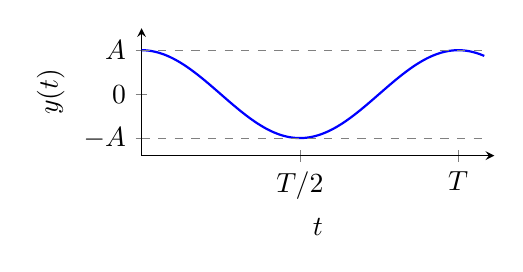
\begin{tikzpicture}
\begin{axis}[
  width=0.5\textwidth, height=3.2cm,
  xlabel={$t$}, ylabel={$y(t)$},
  xmin=0, xmax=7, ymin=-1.4, ymax=1.5,
  xtick={3.1416, 6.2832},
  xticklabels={$T/2$, $T$},
  ytick={-1,0,1}, yticklabels={$-A$,$0$,$A$},
  axis lines=left, samples=200,
]
  \addplot[thick,blue,domain=0:6.8]{cos(deg(x))};
  \draw[dashed,gray] (axis cs:0,1)--(axis cs:6.8,1);
  \draw[dashed,gray] (axis cs:0,-1)--(axis cs:6.8,-1);
\end{axis}
\end{tikzpicture}
\end{center}
\caption{Sinusoidal oscillation with amplitude $A$ and period $T = 2\pi/\omega$.}
\label{fig:shm_cos_ch5}
\end{figure}

\begin{example}[Pendulum with Spring]
A pendulum of length $L$ and mass $m$, with a horizontal spring of spring constant $k$ attached at the pivot end. Find the period of oscillation.

\textbf{Assumptions}: $F_{\text{spring}} = 0$ when $\theta = 0$; small-amplitude oscillations so spring stays horizontal.

Equations of motion in polar coordinates ($r = L = \text{const}$, $\dot{r} = 0$, $\ddot{r} = 0$):

$\hat{r}$-direction:
\[
    mg\cos\theta - T - kx\sin\theta = ma_r = m(\ddot{r} - r\dot{\theta}^2)
\]

$\hat{\theta}$-direction:
\[
    -mg\sin\theta - kx\cos\theta = ma_\theta = m(2\dot{r}\dot{\theta} + r\ddot{\theta})
\]

Small angle: $\sin\theta \approx \theta$, $\cos\theta \approx 1$, $x \approx L\theta$:
\[
    -mg\theta - kL\theta = mL\ddot{\theta}
    \implies -(mg + kL)\theta = mL\ddot{\theta}
\]
\[
    -\left(\frac{g}{L} + \frac{k}{m}\right)\theta = \ddot{\theta}
\]
\[
    \omega = \sqrt{\frac{g}{L} + \frac{k}{m}}
\]
\begin{formula}[Pendulum + Spring Period]
\[
    T = \frac{2\pi}{\sqrt{\dfrac{g}{L} + \dfrac{k}{m}}}
\]
\end{formula}

Check: as $k \to 0$, $\omega \to \sqrt{g/L}$. \checkmark
\end{example}

%───────────────────────────────────────────────────────────────
\section{Conservation of Momentum}
%───────────────────────────────────────────────────────────────

\begin{theorem}[Conservation of Momentum]
For a system with no external forces, $\dv{\vect{P}}{t} = \vect{0}$, so $\vect{P}$ is conserved.
\end{theorem}

Application: measuring the speed of a bullet with little equipment (ballistic pendulum).

\begin{example}[Ballistic Pendulum / Bullet into Block]
A bullet of mass $m$ moving at $v_0$ embeds in a block of mass $M$ on a spring.

Before collision: $\vect{P}_i = mv_0$.

After collision: $\vect{P}_f = (m+M)\vect{v}_i$ (bullet+block move together, spring releases).

By conservation of momentum:
\[
    v_i = \frac{m}{m+M}v_0
\]

The block+bullet then oscillate on the spring:
\[
    -kx = (m+M)\ddot{x}, \quad \omega = \sqrt{\frac{k}{m+M}}
\]
\[
    x(t) = A\cos(\omega t + \phi)
\]
Initial conditions: $x = 0$, $\dot{x} = v_i$ at $t=0$:
\[
    A\cos\phi = 0 \implies \phi = \pi/2
\]
\[
    \dot{x}(0) = v_i = A\omega\cos(0) \implies A = \frac{v_i}{\omega}
\]
\[
    x(t) = \frac{v_i}{\omega}\sin(\omega t)
\]
Maximum distance occurs at $\sin(\omega t) = 1$, i.e.\ $\omega t = \pi/2$:
\[
    x_{\max} = \sqrt{\frac{m+M}{k}}\cdot\frac{m}{m+M}v_0
\]
\[
    v_0 = \frac{\sqrt{k(m+M)}}{m}\,x_{\max}
\]
\end{example}

\begin{example}[Bouncing Ball (Impulse)]
A ball of mass $m$ bouncing off a floor at speed $v$:
\[
    \vect{P}_{\text{before}} = -mv\,\hat{y}, \qquad \vect{P}_{\text{after}} = mv\,\hat{y}
\]
\[
    \Delta\vect{p} = 2mv\,\hat{y}
\]
There is a (large) normal force from the floor. We introduce \emph{impulse}.

Numerical example: $m = 0.2\ \text{kg}$, $v = 8\ \text{m/s}$, contact time $\Delta t = 10^{-3}\ \text{s}$:
\[
    \bar{F} = \frac{2mv}{\Delta t} = \frac{2(0.2)(8)}{10^{-3}} = 3200\ \text{N}
\]
\end{example}

%───────────────────────────────────────────────────────────────
\chapter{Impulse}
%───────────────────────────────────────────────────────────────

\textit{(Saturday, October 21, 2023)}

\section{Impulse}

Given $\vect{F} = \dv{\vect{p}}{t} = m\dv{\vect{v}}{t}$:
\[
    \int_0^t \vect{F}\,dt = \vect{P}(t) - \vect{P}(0)
\]

\begin{definition}[Impulse]
    \[
        \vect{J} = \int_{t_1}^{t_2}\vect{F}\,dt = \int_{t_1}^{t_2}\dv{\vect{p}}{t}\,dt = \vect{p}(t_2) - \vect{p}(t_1) = \Delta\vect{p}
    \]
\end{definition}

When the exact force is not known, it is useful to find the \textbf{average force}:
\[
    F_{\text{av}}\,\Delta t = \int_{t_0}^{t_0+\Delta t}\vect{F}\,dt = \vect{P}(t_0+\Delta t) - \vect{P}(t_0)
\]

\begin{fact}[Gravity and Impulse]
Gravity does create a net impulse, but it is often negligible for short times with high collision forces. Sometimes reframing the situation to remove internal considerations helps.
\end{fact}

\begin{example}[Avoiding Broken Ankles (Landing Force)]
A person falls from height $h$ and decelerates over a distance $s$ (bending knees).

Using kinematics: $v_0 = \sqrt{2gh}$ (speed just before landing). Deceleration phase: $s = \frac{1}{2}a(\Delta t)^2$, $v_0 = a\Delta t$, so $\Delta t = \frac{2s}{v_0}$.

Force during landing:
\[
    F = \frac{Mv_0}{\Delta t} = \frac{Mv_0^2}{2s} \implies F = Mg\frac{h}{s}
\]
Force is linearly proportional to height and inversely to stopping distance --- not an obvious result!
\end{example}

\section{Momentum and Flow of Mass}

Things get tricky when masses combine or explode. Use:
\[
    \int_{t_a}^{t_b}\vect{F}\,dt = \vect{P}(t_b) - \vect{P}(t_a)
\]

\begin{example}[Freight Car and Hopper (Mass Accretion)]
Consider a small time interval $\Delta t$. A hopper drops mass $\Delta m$ (at rest) onto a freight car of mass $M$ moving at velocity $v$.

\[
    P_i = 0 + Mv, \qquad P_f = (M + \Delta m)v
\]
\[
    \Delta P = P_f - P_i = (M + \Delta m)v - Mv = \Delta m\,v
\]
\[
    \frac{\Delta P}{\Delta t} = \frac{\Delta m}{\Delta t}v \implies \dv{P}{t} = \frac{dm}{dt}v = F
\]
For the leaking sand case (mass leaving): $F = 0$ (no external horizontal force).
\end{example}

\begin{fact}[Common Error in Variable-Mass Problems]
Do NOT write:
\[
    F = \dv{p}{t} = \dv{}{t}(mv) = m\dv{v}{t} + v\cdot\dv{m}{t}
\]
This is \textbf{wrong} when $dm/dt \neq 0$, because the second term $v\,\dv{m}{t}$ double-counts momentum. Use impulse--momentum applied to a well-defined system boundary instead.
\end{fact}

%───────────────────────────────────────────────────────────────
\section{Rocket Motion}
%───────────────────────────────────────────────────────────────

A rocket expels mass $\Delta m$ during a time interval $\Delta t$ at exhaust velocity $\vect{u}$ relative to the rocket.

\begin{figure}[H]
\begin{center}
\begin{tikzpicture}[scale=0.95, >=Stealth]
  % === Before (top) ===
  \node[left] at (-0.2,2.5) {\small\textbf{time $t$:}};
  % Rocket body
  \fill[gray!30] (0.5,2.1) rectangle (2.5,2.9);
  \draw[thick] (0.5,2.1) -- (2.5,2.1) -- (2.5,2.9) -- (0.5,2.9) -- cycle;
  \draw[thick] (2.5,2.5) -- (3.0,2.5);  % nozzle
  % Nose cone
  \fill[gray!50] (0.0,2.5) -- (0.5,2.1) -- (0.5,2.9) -- cycle;
  \node at (1.5,2.5) {$M$};
  % Velocity arrow
  \draw[->,thick,blue] (3.0,2.5) -- (4.2,2.5) node[right]{$v$};

  % === After (bottom) ===
  \node[left] at (-0.2,0.8) {\small\textbf{time $t+\Delta t$:}};
  % Rocket body (lighter)
  \fill[gray!30] (0.5,0.4) rectangle (2.2,1.2);
  \draw[thick] (0.5,0.4) -- (2.2,0.4) -- (2.2,1.2) -- (0.5,1.2) -- cycle;
  \draw[thick] (2.2,0.8) -- (2.6,0.8);
  \fill[gray!50] (0.0,0.8) -- (0.5,0.4) -- (0.5,1.2) -- cycle;
  \node at (1.35,0.8) {$M{-}\Delta m$};
  % Rocket velocity
  \draw[->,thick,blue] (2.6,0.8) -- (3.9,0.8) node[right]{$v{+}\Delta v$};
  % Exhaust gas
  \fill[orange!40] (2.8,0.55) rectangle (3.8,0.35);
  \draw[thick,orange] (2.8,0.55) rectangle (3.8,0.35);
  \node[below,orange,scale=0.8] at (3.3,0.35) {$\Delta m$};
  \draw[->,thick,orange] (2.8,0.45) -- (1.8,0.45) node[left,scale=0.8]{exhaust $u$};
\end{tikzpicture}
\end{center}
\caption{Rocket of mass $M$ moving at $v$ (top). After $\Delta t$ (bottom): rocket has mass $M-\Delta m$ at speed $v+\Delta v$, expelled gas $\Delta m$ moves backward at exhaust speed $u$ relative to rocket.}
\label{fig:rocket}
\end{figure}

\[
    p(t) = (M + \Delta m)v
\]
\[
    p(t+\Delta t) = (v+\Delta v)M + \Delta m(v + \Delta v + u)
\]
\[
    p(t+\Delta t) - p(t) = MV + M\Delta v + \Delta m\,v + \Delta m\,\Delta v + \Delta m\,u - Mv - \Delta m\,v
    = M\Delta v + \Delta m(\Delta v + u)
\]

As $\Delta t \to 0$, the non-first-order term $\Delta m\,\Delta v$ vanishes (\textbf{Physics Tip: non-first-order terms vanish in the limit}):
\[
    \dv{p}{t} = M\dv{v}{t} + \frac{dm}{dt}\cdot u
\]

By conservation of momentum (no external force): with mass conservation $\dv{M}{t} = -\dv{m_{\text{exhaust}}}{t}$:

\begin{formula}[Rocket Equation]
\[
    M\dv{v}{t} = -u\dv{M}{dt} = u\dv{m_{\text{exhaust}}}{dt}
\]
\end{formula}

\subsection{Integrating the Rocket Equation}

\[
    \dv{v}{t} = \frac{u}{M}\dv{M}{dt}
\]
\[
    \int_{t_0}^{t_f}\dv{v}{t}\,dt = u\int_{M_0}^{M_f}\frac{1}{M}\,dM
\]
\[
    v_f - v_0 = u\ln\frac{M_f}{M_0} = -u\ln\!\left(\frac{M_0}{M_f}\right)
\]

\begin{formula}[Tsiolkovsky Rocket Equation (No Gravity)]
If $v_0 = 0$:
\[
    v_f = -u\ln\!\left(\frac{M_0}{M_f}\right) = u\ln\!\left(\frac{M_0}{M_f}\right)
\]
(taking $u$ as the magnitude of exhaust speed, with exhaust directed backward).
\end{formula}

\textbf{Including gravity}:
\[
    Mg = M\dv{v}{t} - u\dv{M}{dt} \quad (\text{thrust} = u\dv{M}{dt})
\]
\[
    \dv{v}{t} = \frac{u}{M}\dv{M}{dt} + g
\]
Integrating:
\[
    \int_{v_0}^{v_f}dv = u\int_{M_0}^{M_f}\frac{1}{M}\,dM + g\Delta t
\]
\begin{formula}[Rocket Equation with Gravity]
\[
    v_f = -u\ln\!\left(\frac{M_f}{M_0}\right) + g t_f \quad (v_0 = 0)
\]
\end{formula}

%───────────────────────────────────────────────────────────────
\chapter{Momentum Flow, Force, and Work-Energy Theorem}
%───────────────────────────────────────────────────────────────

\section{Momentum Flow and Force}

\textit{(Thursday, October 26, 2023)}

Consider the impulse of catching a small droplet of water ($v_f = 0$):
\[
    I_{\text{droplet}} = \int_{\text{collision}} F\,dt = \Delta p = m(v_f - v) = -mv
\]
So impulse on droplet $= -mv$. By Newton's 3rd law:
\[
    I_{\text{nozzle}} = mv
\]
If there are multiple collisions per second (period $T$ between collisions):
\[
    F_{\text{av}}\cdot T = \int_{\text{collision}} F\,dt = mv
\]
\begin{formula}[Average Force from Droplet Stream]
\[
    F_{\text{av}} = \frac{mv}{T} = \frac{mv^2}{\ell}, \quad \ell = vT
\]
(Note: this is the same form as the centripetal force $mv^2/r$ in circular motion!)
\end{formula}

\section{Momentum Flux}

\begin{definition}[Momentum Flux]
The average momentum per unit length is $mv/\ell$. The momentum flux (rate of momentum transport) is:
\[
    \frac{mv}{\ell}\cdot v = \frac{mv^2}{\ell} = \frac{mv}{T}
\]
For a continuous stream of matter with cross-sectional area $A$, speed $v$, in direction $\hat{v}$, and mass density $\rho_m$:
\[
    \dot{\vect{p}} = \rho_m v^2 A\,\hat{v}
\]
where $\dot{\vect{p}}$ is the rate at which momentum flows through a hypothetical surface across the stream.
\end{definition}

\begin{figure}[H]
\begin{center}
\begin{tikzpicture}[scale=0.9, >=Stealth]
  % Surface (vertical wall)
  \fill[pattern=north east lines] (3.5,-0.5) rectangle (3.8,1.5);
  \draw[thick] (3.5,-0.5) -- (3.5,1.5);
  % Stream arrows (flow to right)
  \foreach \y in {0.1, 0.5, 0.9} {
    \draw[->,thick,blue] (0.3,\y) -- (2.5,\y);
    \fill[blue!30] (0.5,\y-0.12) rectangle (1.8,\y+0.12);
  }
  \node[above] at (1.3,1.1) {$\rho,\, v$};
  % Cross section label
  \draw[<->] (0.3,-0.3) -- (0.3,1.1) node[midway,left]{$A$};
  % Force on wall
  \draw[->,thick,red] (3.5,0.5) -- (4.5,0.5) node[right]{$\dot{p} = \rho v^2 A$};
\end{tikzpicture}
\end{center}
\caption{A stream of matter (density $\rho$, speed $v$, cross-section $A$) impinges on a surface. The momentum flux $\dot{p} = \rho v^2 A$ is the force exerted on the surface.}
\label{fig:momentum_flux}
\end{figure}

By Newton's 3rd law, the force on the surface on the stream is:
\[
    \vect{P}_{\text{surface on stream}} = -\rho_m v^2 A\,\hat{v}
\]

\begin{example}[Lennard-Jones Force (Momentum Flux Context)]
The Lennard-Jones potential between two particles separated by $r$:
\[
    V(r) = 4\varepsilon\left[\left(\frac{\sigma}{r}\right)^{12} - \left(\frac{\sigma}{r}\right)^6\right]
\]
The corresponding force:
\begin{align*}
    F(r) &= -\dv{V}{r} = 4\varepsilon\left(\frac{-12\sigma^{12}}{r^{13}} + \frac{6\sigma^6}{r^7}\right) \\
    &= 48\varepsilon\left(\frac{\sigma^{12}}{r^{13}} - \frac{\sigma^6}{2r^7}\right)
\end{align*}
Let $\beta = \sigma^6/r^6$:
\[
    = \frac{48\varepsilon}{r}\beta\left(\beta - \frac{1}{2}\right)
\]
\begin{formula}[Lennard-Jones Force]
\[
    F(r) = \frac{48\varepsilon}{r}\,\beta\!\left(\beta - \frac{1}{2}\right), \quad \beta = \frac{\sigma^6}{r^6}
\]
\end{formula}
\end{example}

%───────────────────────────────────────────────────────────────
\chapter{Work and Energy}
%───────────────────────────────────────────────────────────────

\textit{(Energy 2, Tuesday October 24, 2023)}

\section{Work-Energy Theorem (Review)}

\begin{formula}[Work-Energy Theorem]
\[
    W = \int_{x_i}^{x_f} F\,dx = \frac{1}{2}mv_f^2 - \frac{1}{2}mv_i^2
\]
\end{formula}

\begin{example}[Ball Under Gravity — Two Methods]
A ball thrown upward at speed $v_0$. Maximum height $h$:

\textbf{Kinematics}: $t_f = v_0/g$, $h = -\frac{1}{2}g(v_0/g)^2 + v_0(v_0/g) = \frac{v_0^2}{2g}$.

\textbf{Work-energy}:
\[
    \int_0^h F\,dx = \int_0^h (-mg)\,dx = -mgh = \frac{1}{2}m(v_f^2 - v_i^2) = -\frac{1}{2}mv_0^2
\]
\[
    \implies h = \frac{v_0^2}{2g} \quad \checkmark
\]
\end{example}

\begin{example}[Falling Weight Demo]
A mass falls from height $h$. Work-energy gives:
\[
    \int_h^0 (-mg)\,dx = \frac{1}{2}m(v_f^2 - v_0^2)
\]
\[
    mgh = \frac{1}{2}mv_f^2 \implies v_f = \sqrt{2gh}
\]
For the pendulum: the tension does no work since $\vect{T}\perp\dot{\vect{x}}$.
\end{example}

\begin{example}[Escape Velocity]
What velocity is needed for a projectile to escape Earth's gravitational field? (Escape from radius $r_e$, $v_f \to 0$ at $r \to \infty$.)
\[
    \int F\,dx = -GmM\int_{r_e}^{\infty}\frac{dr}{r^2} = \frac{1}{2}mv_f^2 - \frac{1}{2}mv_i^2
\]
\[
    -\frac{GmM}{r_e} = -\frac{1}{2}mv_i^2 \quad (\text{to escape, }\tfrac{1}{2}mv_f^2 > 0)
\]
\[
    \frac{1}{2}mv_i^2 - \frac{GmM}{r_e} > 0 \implies v_i^2 > \frac{2GM}{r_e}
\]
\begin{formula}[Escape Velocity]
\[
    v_i > \sqrt{\frac{2GM}{r_e}}
\]
\end{formula}
\end{example}

\begin{example}[Spring and SHO via Work-Energy]
$\Delta x = A\cos(\omega t + \phi)$, $\phi = \pi/2$ (from $x=0$ initial condition):
\[
    \int_0^{x_f} F\,dx = -\int_0^{x_f} kx\,dx = -\frac{1}{2}kx_f^2
\]
\[
    -\frac{1}{2}kx_f^2 = \frac{1}{2}mv_f^2 - \frac{1}{2}mv_i^2 \implies kx_f^2 = mv_i^2
\]
\[
    x_f = \sqrt{\frac{m}{k}}\,v_i \quad \checkmark
\]
\end{example}

\section{Definitions: Energy}

\begin{definition}[Kinetic Energy]
    \[
        KE = \frac{1}{2}mv^2 \quad \text{(valid only at non-relativistic speeds)}
    \]
\end{definition}

\begin{definition}[Potential Energy]
\begin{itemize}
    \item Constant gravity: $U = mgh$
    \item Varying gravity: $U = -\displaystyle\int_{r_i}^{r_f}\frac{GmM}{r^2}\,dr$
    \item Spring: $U = \frac{1}{2}k\Delta x^2$
\end{itemize}
\end{definition}

\begin{formula}[Work-Energy Theorem (General)]
\[
    W = \int \vect{F}\cdot d\vect{r} = \frac{1}{2}mv_f^2 - \frac{1}{2}mv_i^2 = \Delta KE
\]
\end{formula}

\textbf{Extension to 3D}:
\[
    W = \int_C \vect{F}\cdot d\vect{r} \quad (C: \text{ curve of path})
\]

\begin{definition}[Power]
    \[
        P = \dv{W}{t} = \vect{F}\cdot\vect{v}
    \]
    Example (power due to gravity on an object moving at angle $\theta$ from horizontal at speed $v_0$):
    \[
        P = mgv_0\cos(\theta + 90°) = -mgv_0\sin\theta
    \]
\end{definition}

\section{Limitations of the Work-Energy Theorem}

\begin{fact}[Work-Energy Theorem Requires Conservative Forces]
The work-energy theorem only works for \textbf{conservative forces}. For a closed path:
\[
    W = \oint \vect{F}\cdot d\vect{r} = 0 \implies \frac{1}{2}mv_f^2 = \frac{1}{2}mv_i^2
\]
This makes sense for gravity (if a ball starts and ends at height $h$, net work by gravity is zero).

\textbf{Friction} is non-conservative: work depends on path length, so it does not conserve mechanical energy. More research needed into friction at the microscopic level.
\end{fact}
